% IRMF talk. Build from overleaf/:  tectonic irmf_talk.tex   (or latexmk -pdf irmf_talk.tex)
% Figures: figures/real-vs-calculated*, figures/real_vs_calculated_slides, figures/irmf-talk (new).
\documentclass[aspectratio=169,14pt]{beamer}
\geometry{paperwidth=254mm,paperheight=142.875mm}
\usepackage{fix-cm}
\DeclareFontShape{OT1}{cmss}{m}{it}{<->ssub*cmss/m/sl}{}
\usepackage{amsmath,amssymb,booktabs,array,graphicx,xcolor}

\definecolor{ink}{HTML}{172B3A}
\definecolor{blue}{HTML}{2563A6}
\definecolor{orange}{HTML}{C65B32}
\definecolor{teal}{HTML}{087F8C}
\definecolor{muted}{HTML}{576B79}
\setbeamercolor{normal text}{fg=ink,bg=white}
\setbeamercolor{frametitle}{fg=ink}
\setbeamercolor{title}{fg=ink}
\setbeamercolor{structure}{fg=blue}
\setbeamercolor{alerted text}{fg=orange}
\setbeamerfont{frametitle}{size=\fontsize{24}{28}\selectfont,series=\bfseries}
\setbeamerfont{title}{size=\fontsize{34}{40}\selectfont,series=\bfseries}
\setbeamersize{text margin left=14mm,text margin right=14mm}
\setbeamertemplate{navigation symbols}{}
\setbeamertemplate{itemize items}[circle]
\setbeamertemplate{frametitle}{\vspace{5mm}\insertframetitle\par\vspace{2mm}}
\setbeamertemplate{footline}{%
    \hfill{\color{muted}\fontsize{9}{11}\selectfont\insertframenumber}\hspace{14mm}\vspace{4mm}}
\graphicspath{{figures/}}
\newcommand{\takeaway}[1]{\par\vspace{2mm}{\color{teal}#1\par}}
\newcommand{\fignote}[1]{\par\vspace{1mm}{\fontsize{10}{12}\selectfont\color{muted}#1\par}}
\newcommand{\plot}[2][72mm]{\par\centering\includegraphics[width=\textwidth,height=#1,keepaspectratio]{#2}\par\raggedright}
\newcommand{\defeq}{\stackrel{\mathrm{def}}{=}}
\newcommand{\RMSE}{\operatorname{RMSE}}
\newcommand{\yes}{{\color{teal}\checkmark}}
\newcommand{\no}{{\color{orange}$\times$}}

\begin{document}

\begin{frame}[plain]
    \vfill
    {\usebeamerfont{title}Intrinsic Robust Multiscale Filtering\par}
    \vspace{6mm}
    {\Large\color{muted}Splitting a signal into scales when the data are contaminated\par}
    \vfill
\end{frame}

\begin{frame}{The problem: signal + noise + contamination}
    \vspace{-3mm}
    \plot[100mm]{irmf-talk/observations_6sigma.pdf}
    \fignote{\(Y_i = X_i + G_i + M_iC_i\): Gaussian noise \(G_i\sim\mathcal N(0,\sigma^2)\); at a random fraction \(p\) of points (\(M_i=1\)) a gross error \(C_i\).
    Goal: recover the coarse-to-fine components of the clean signal \(X\).}
\end{frame}

\begin{frame}{IMF in pictures: a window slides along the series}
    \vspace{-4mm}
    \centering
    \only<1>{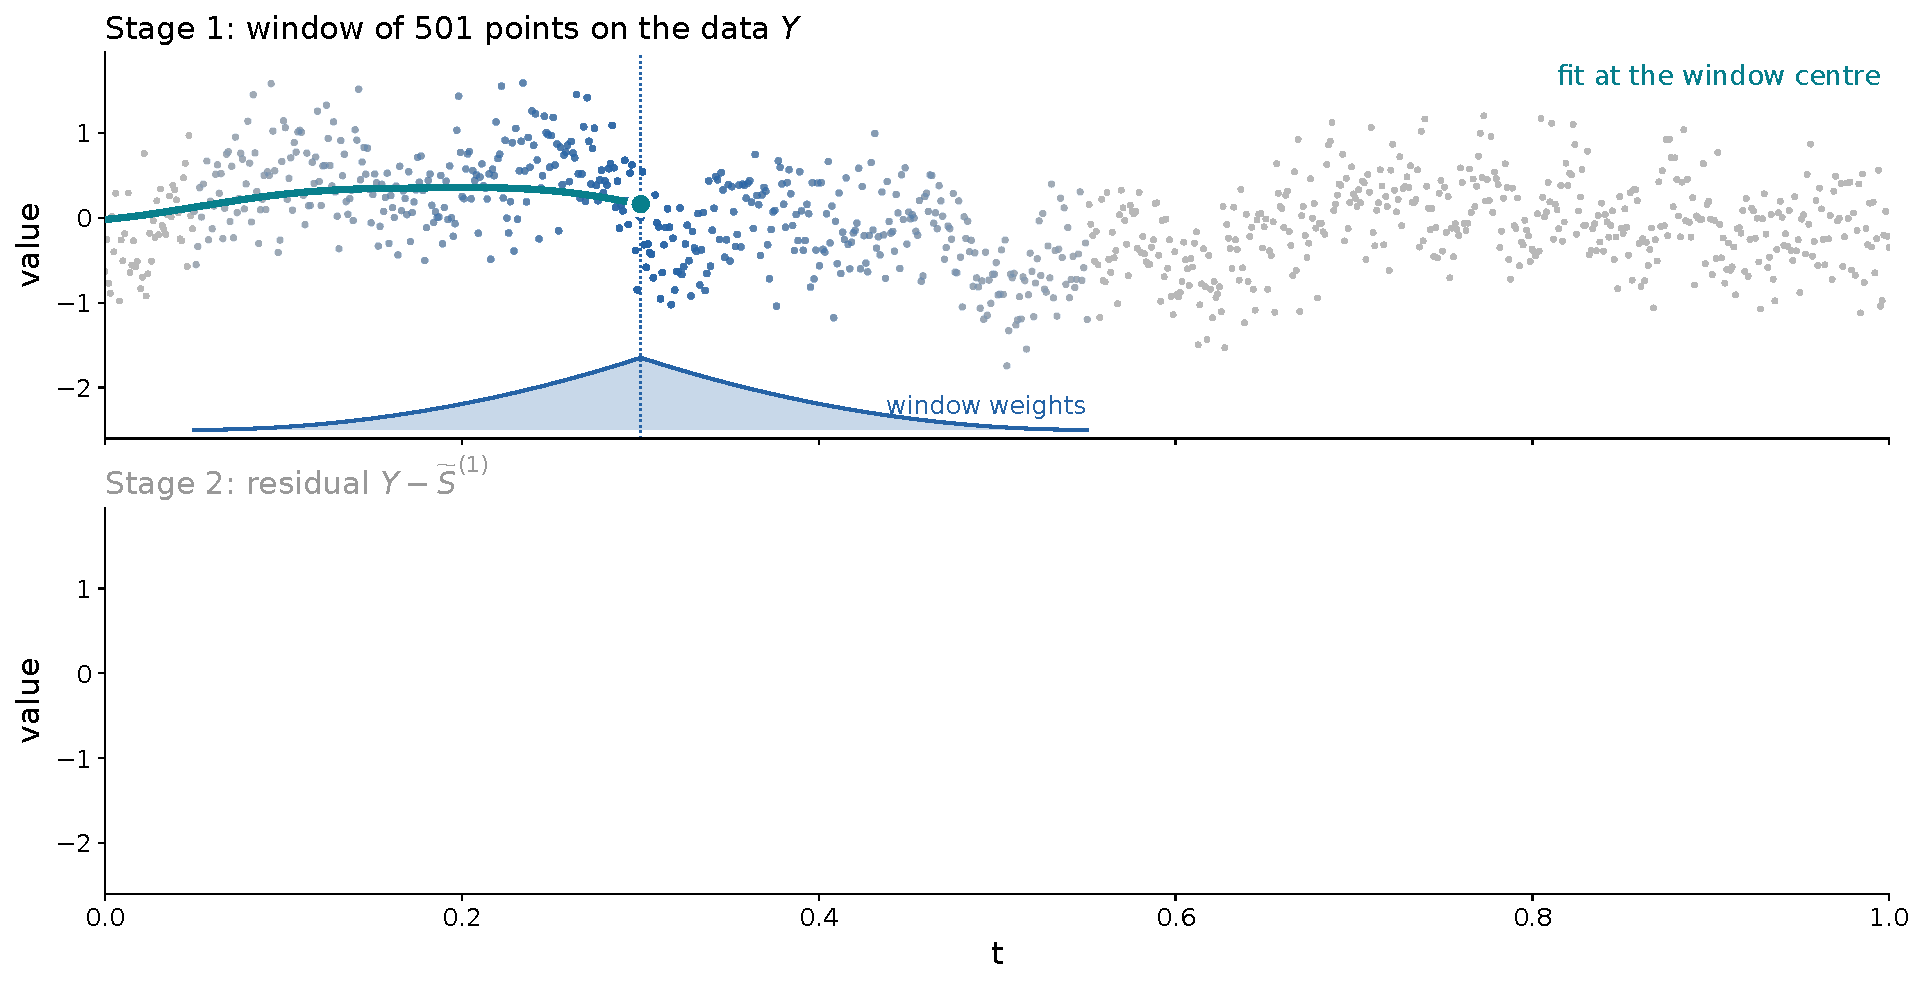
\includegraphics[width=\textwidth,height=96mm,keepaspectratio]{irmf-talk/window_step1.pdf}}
    \only<2>{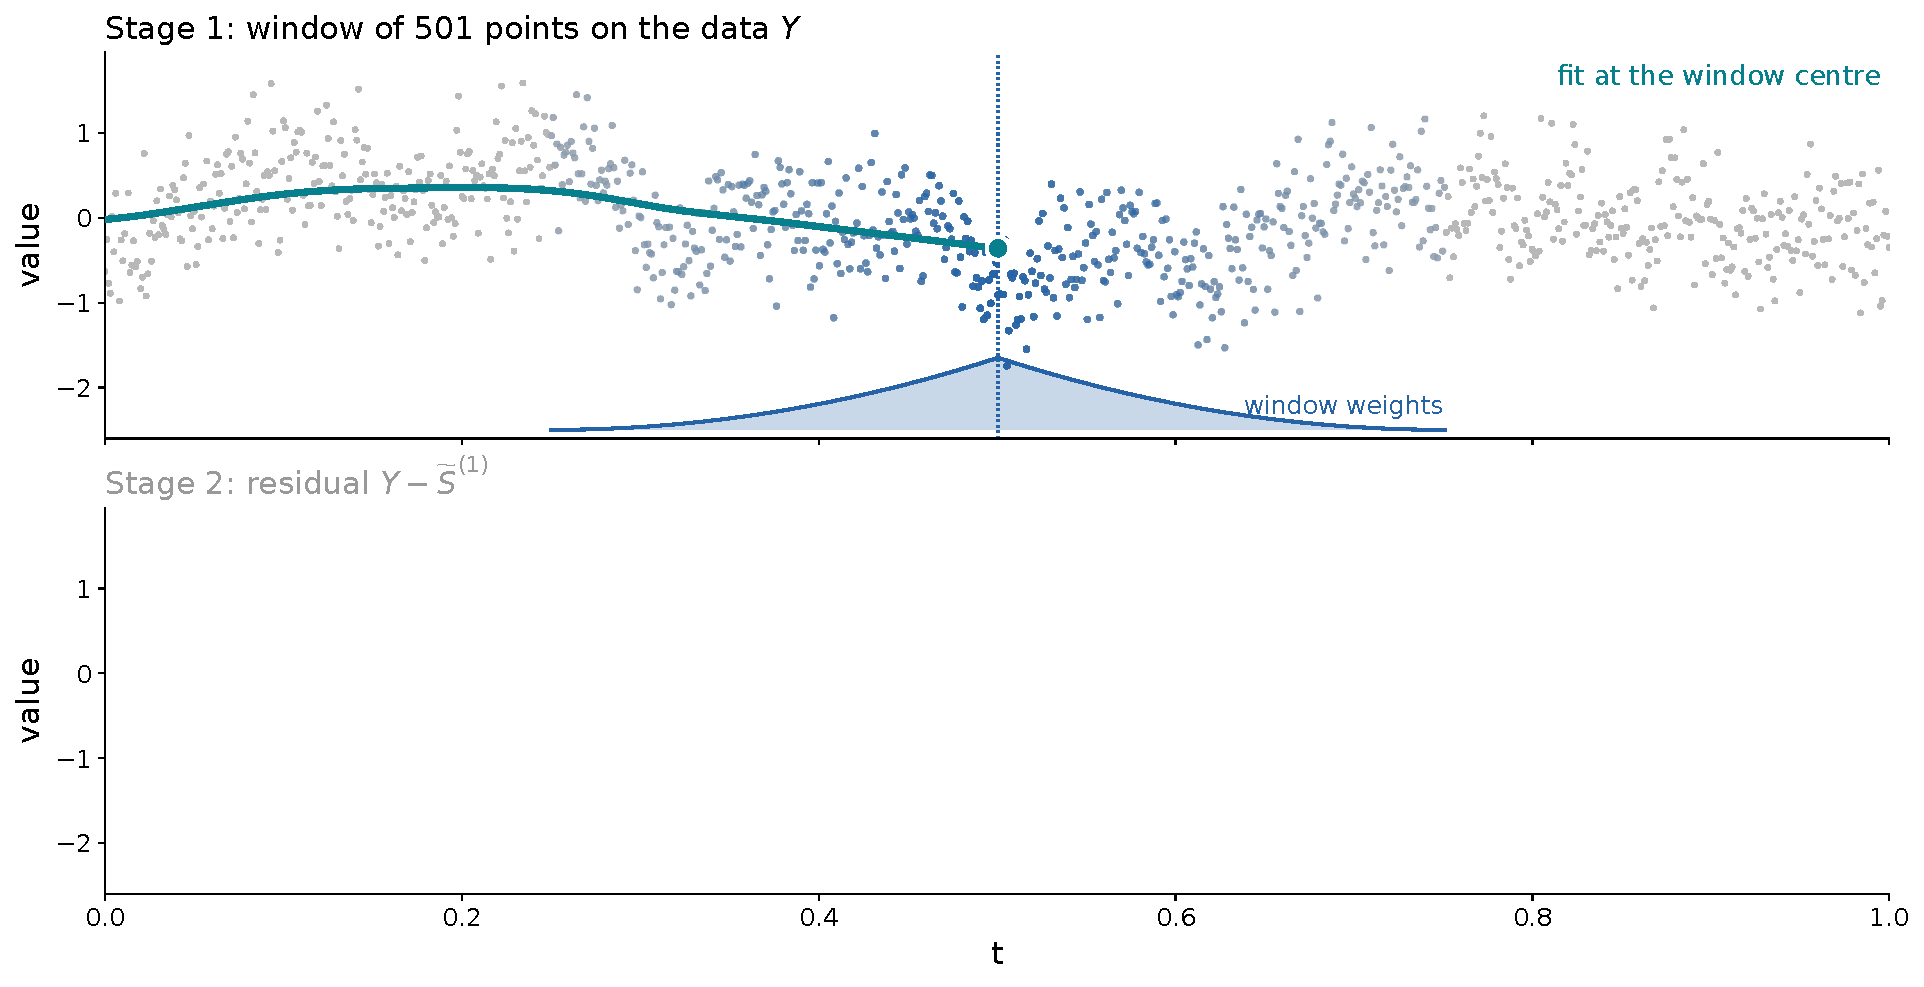
\includegraphics[width=\textwidth,height=96mm,keepaspectratio]{irmf-talk/window_step2.pdf}}
    \only<3>{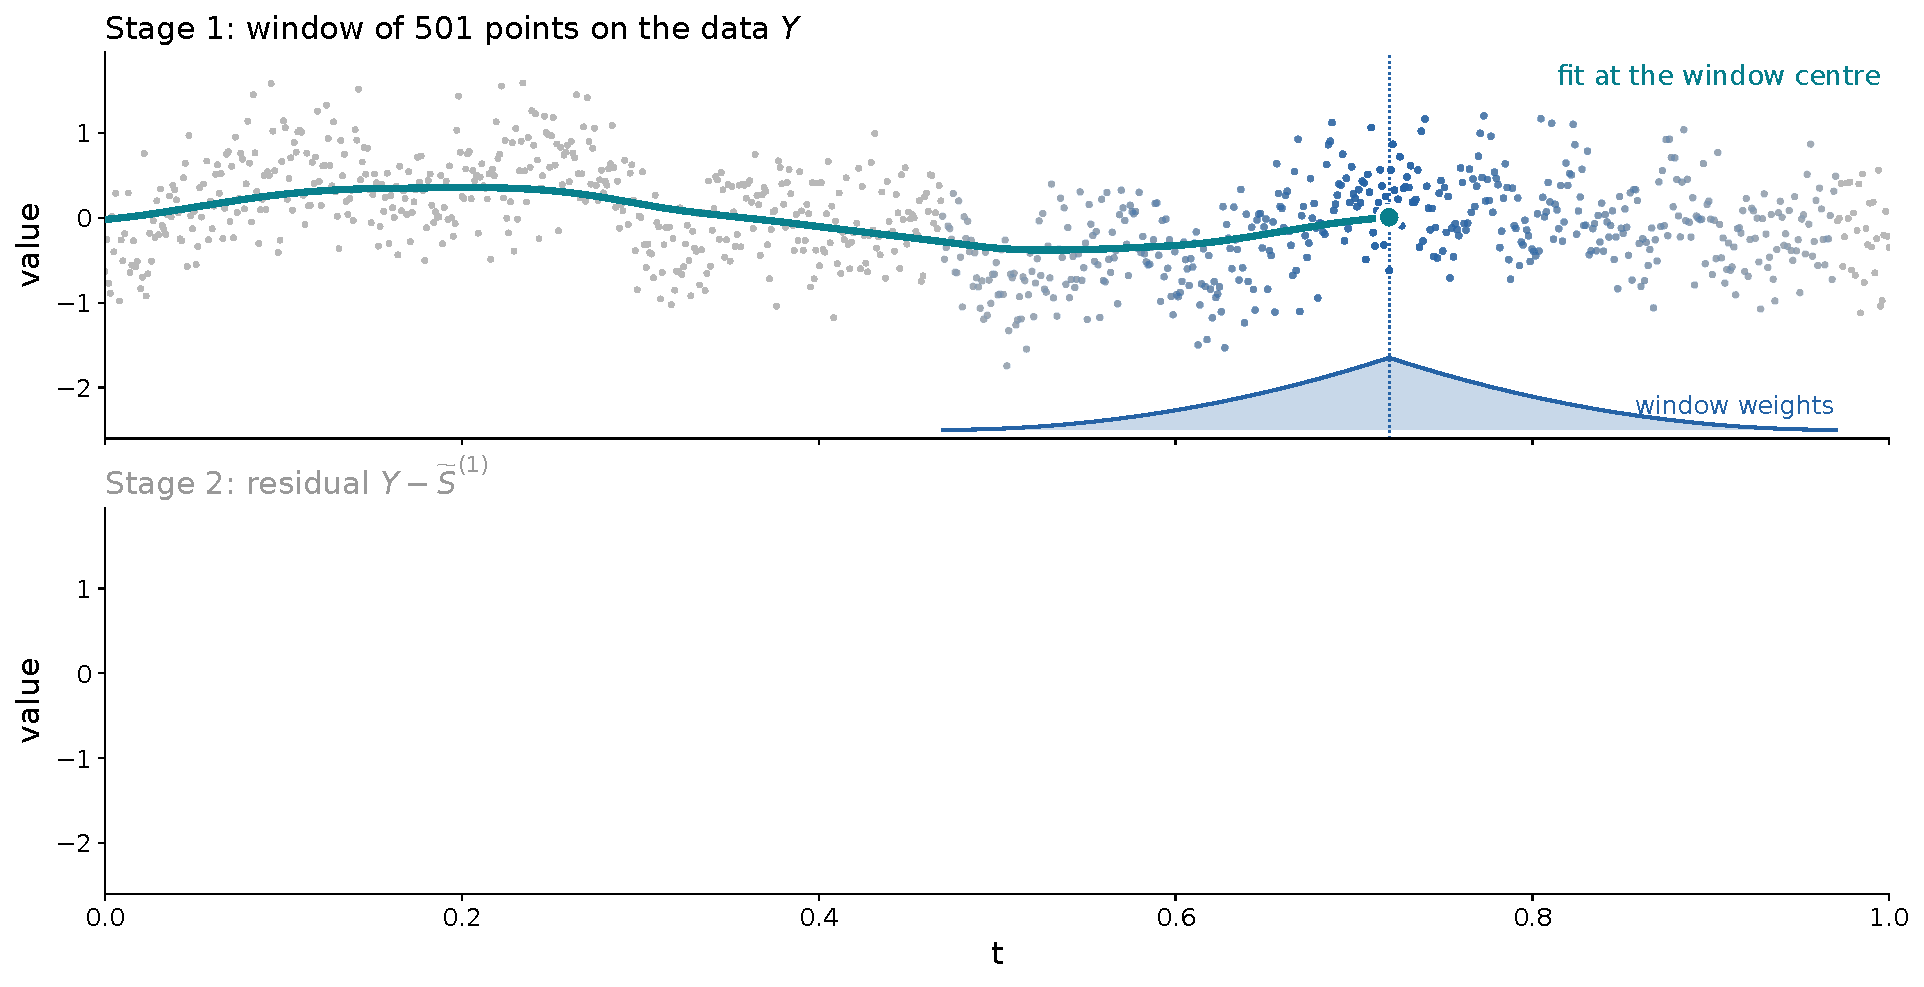
\includegraphics[width=\textwidth,height=96mm,keepaspectratio]{irmf-talk/window_step3.pdf}}
    \only<4>{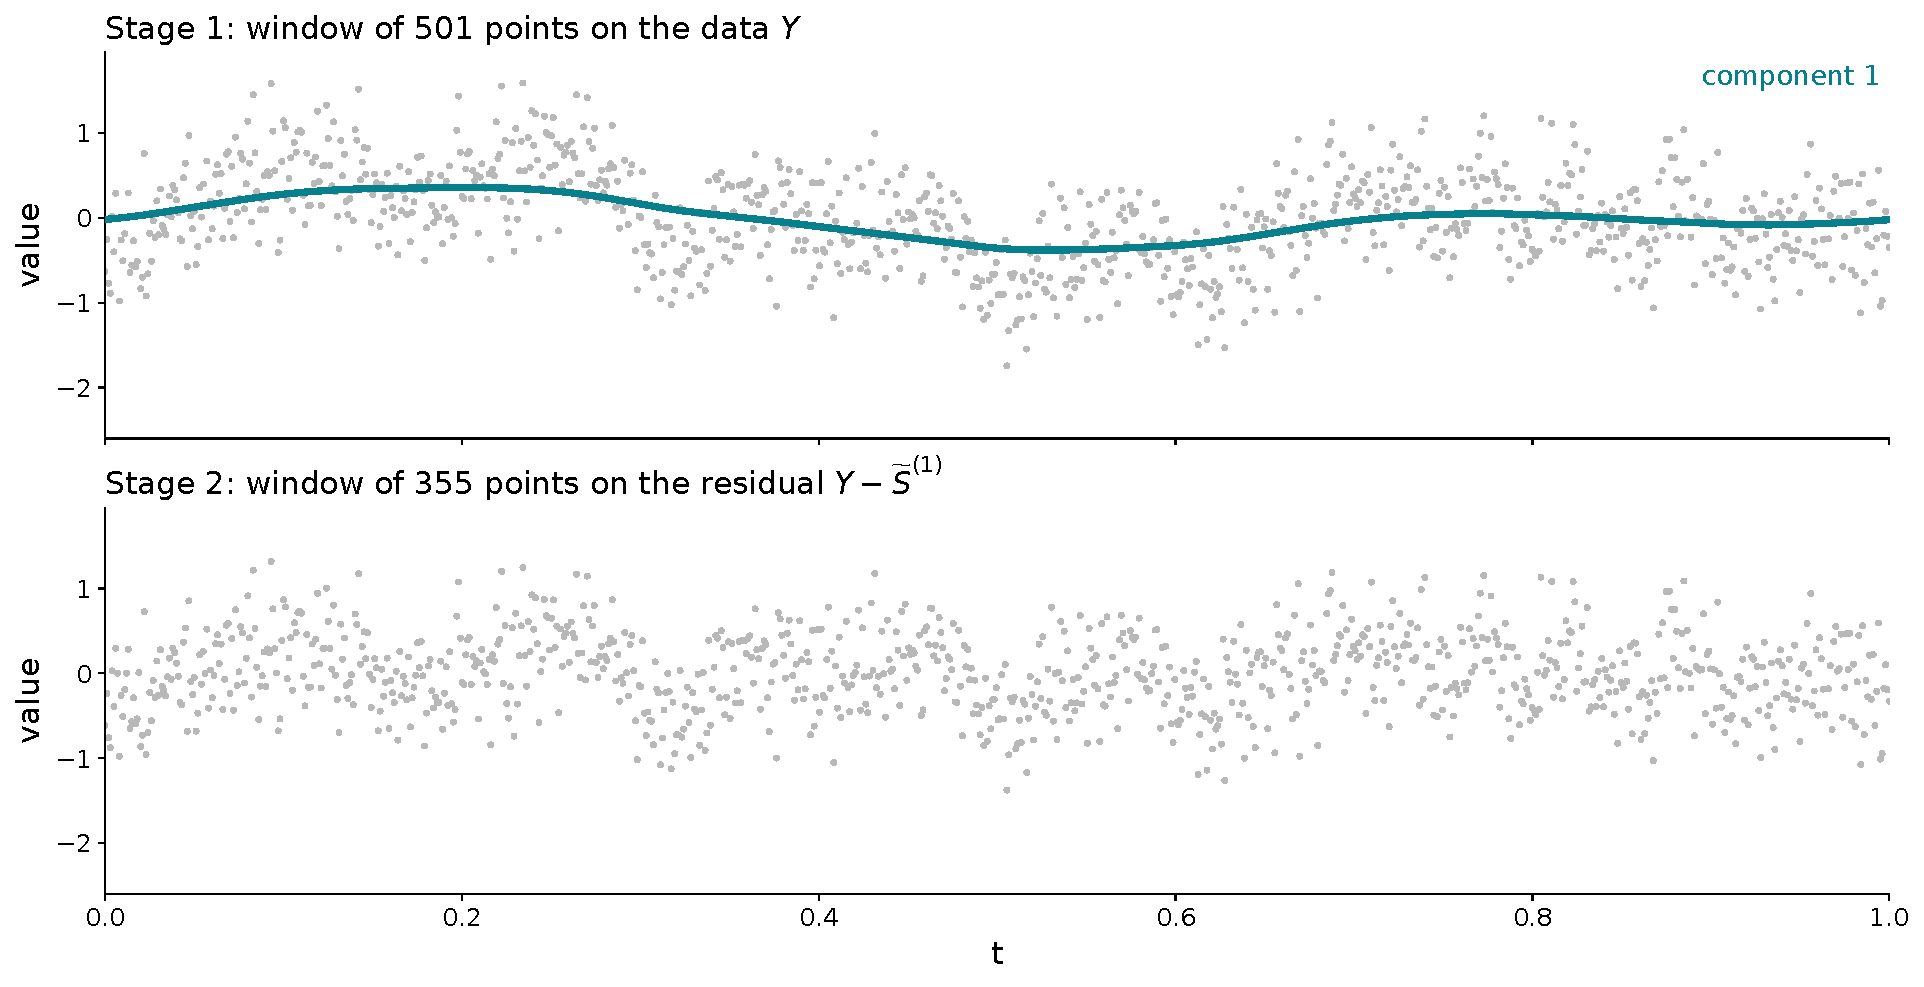
\includegraphics[width=\textwidth,height=96mm,keepaspectratio]{irmf-talk/window_step4.pdf}}
    \only<5>{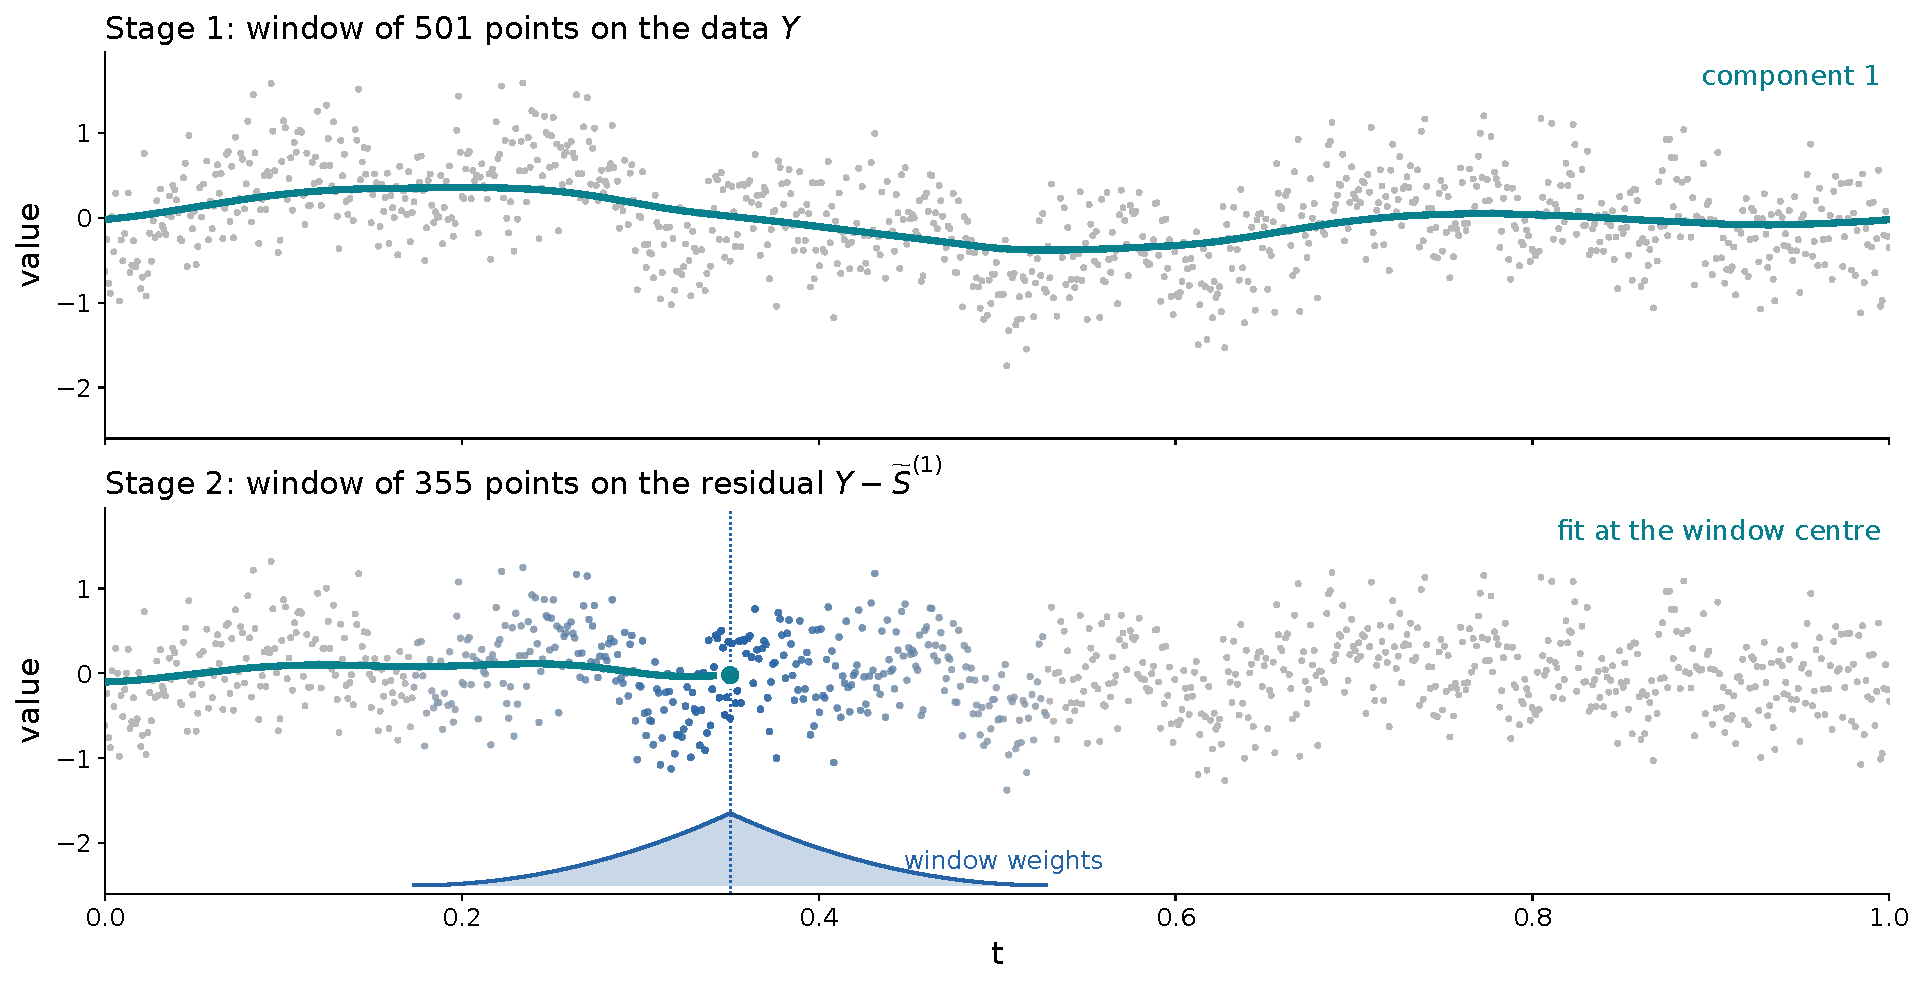
\includegraphics[width=\textwidth,height=96mm,keepaspectratio]{irmf-talk/window_step5.pdf}}
    \only<6>{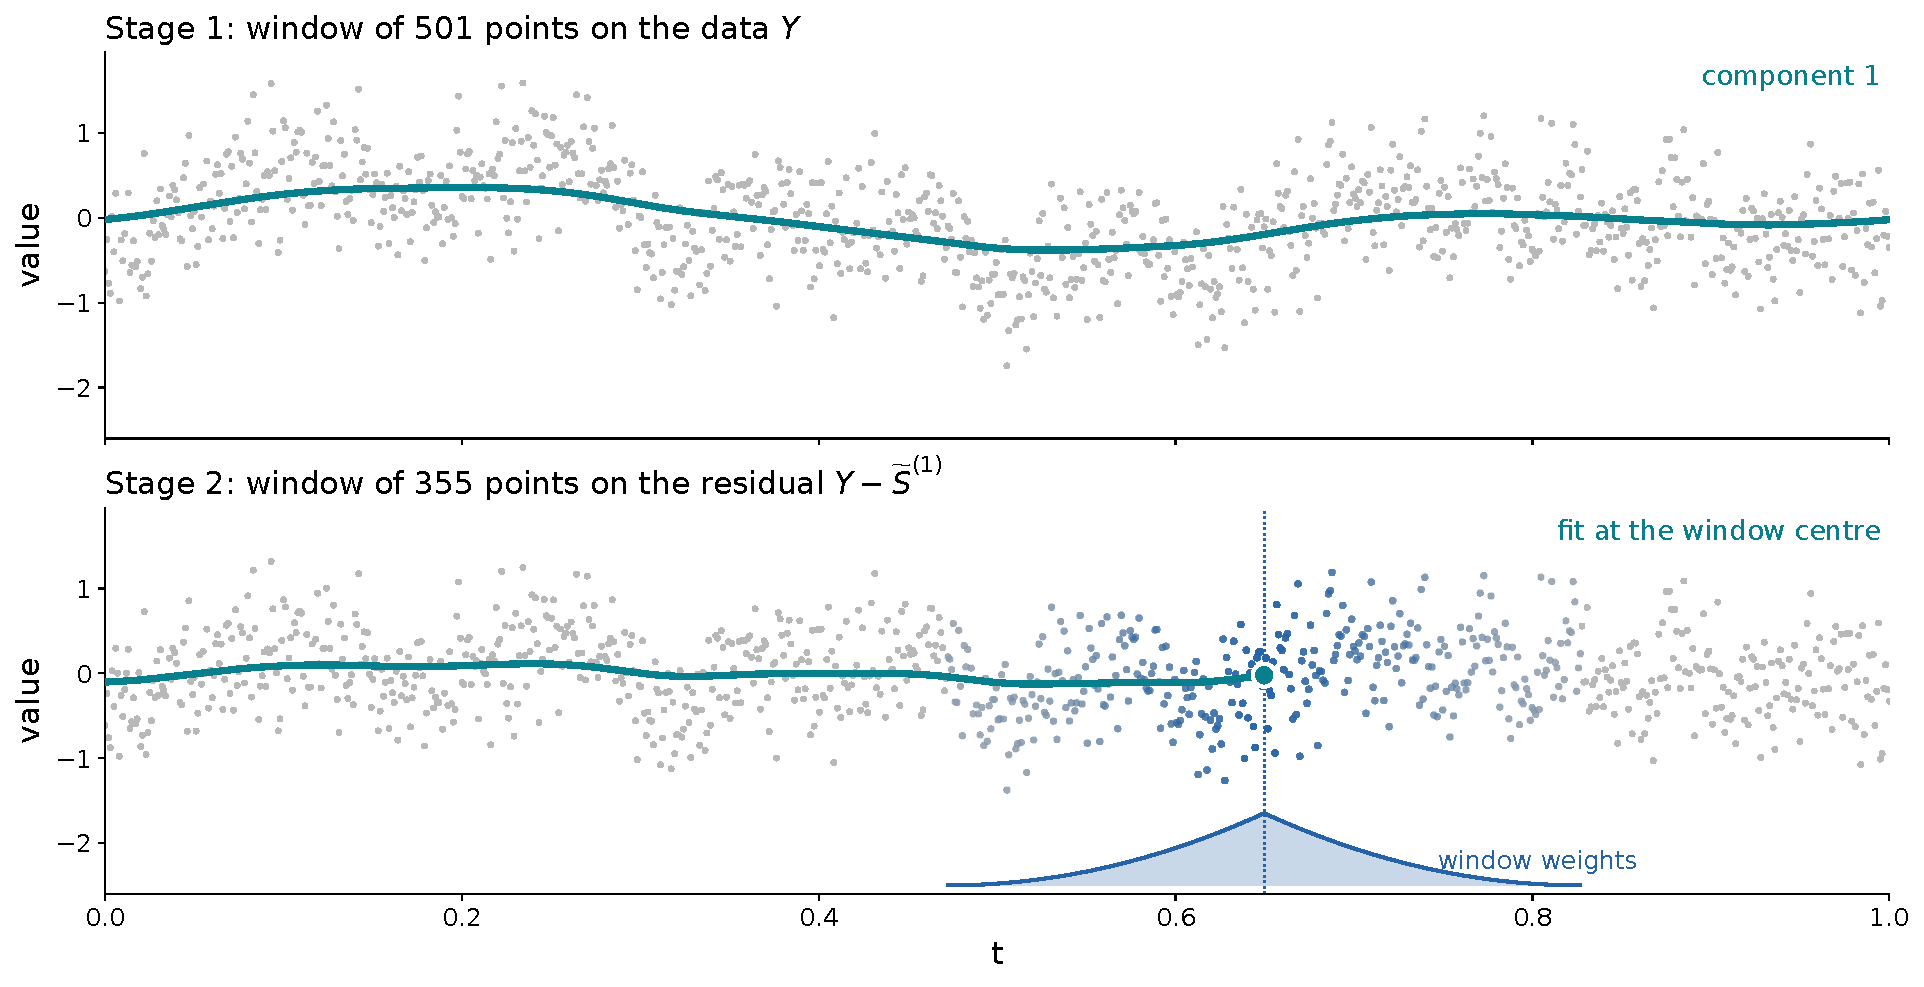
\includegraphics[width=\textwidth,height=96mm,keepaspectratio]{irmf-talk/window_step6.pdf}}
    \only<7>{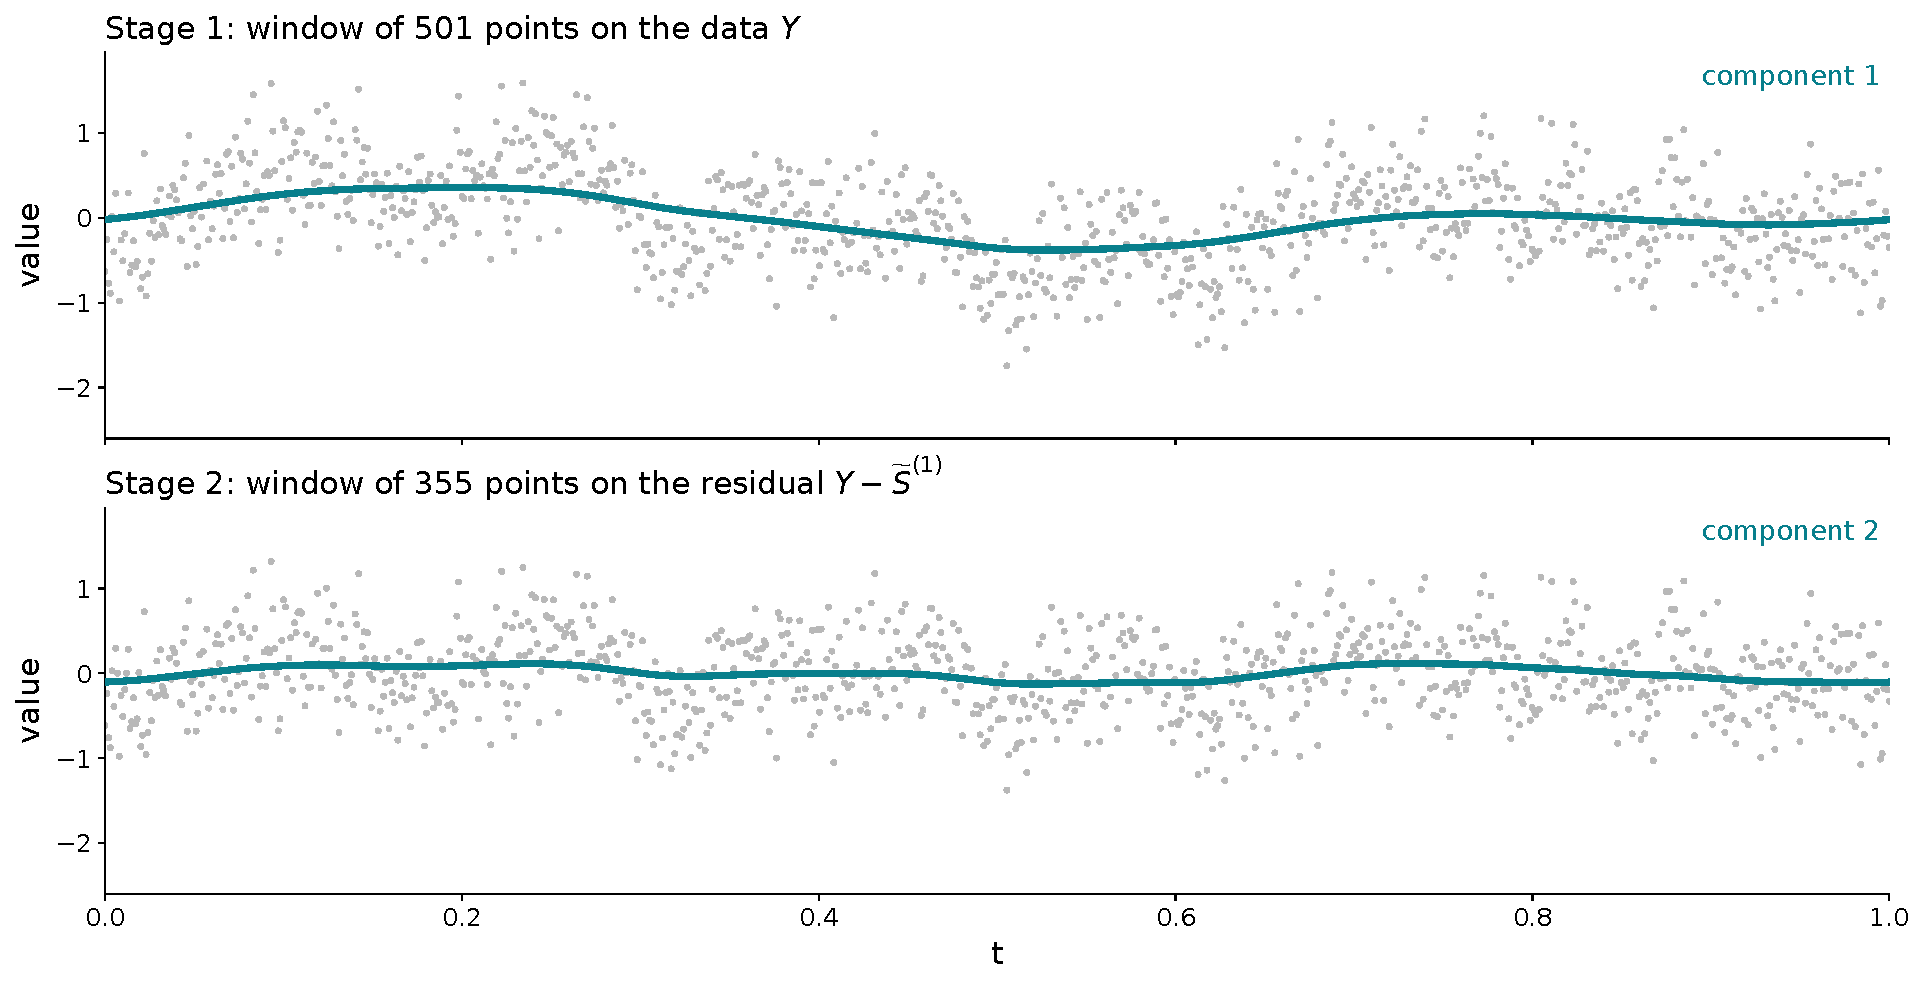
\includegraphics[width=\textwidth,height=96mm,keepaspectratio]{irmf-talk/window_step7.pdf}}
    \par\raggedright\vspace{-1mm}
    \only<1-3>{At each time \(t\), fit one value to the points in the window around \(t\) (darker = more weight). Moving the window traces component 1.}%
    \only<4>{Subtract component 1. What remains is passed to the next stage.}%
    \only<5-6>{Same on the residual, with a window \(a=\sqrt2\) times narrower: component 2.}%
    \only<7>{Repeat with ever narrower windows, 501 \(\to\) 355 \(\to\) 251 \(\to\cdots\to\) 31 points.}
\end{frame}

\begin{frame}{IMF: peel off scales from coarse to fine}
    Start with \(Y^{(1)}\defeq Y\) and a wide window \(h_1\). At stage \(k\):
    \[
        \widetilde S^{(k)}_t\defeq \arg\min_{x}\sum_u \rho\bigl(Y^{(k)}_u-x\bigr)\,K\!\Bigl(\frac{t-u}{h_k}\Bigr),
        \qquad
        Y^{(k+1)}\defeq Y^{(k)}-\widetilde S^{(k)},\qquad h_{k+1}\defeq \frac{h_k}{a}.
    \]
    \vspace{1mm}
    \begin{columns}[T,onlytextwidth]
        \begin{column}{0.44\textwidth}
            {\color{blue}\large Linear IMF}\par
            \[\rho(r)\defeq \tfrac12 r^2 \;\Rightarrow\; \text{local weighted mean}\]
            Every point pulls with strength \(\propto\) its distance.
        \end{column}
        \begin{column}{0.54\textwidth}
            {\color{orange}\large Robust IMF (IRMF)}\par
            \[\rho_H(r)\defeq \mathbb E\,|r+H\xi|,\qquad \psi_H(r)\defeq \rho_H'(r),\quad |\psi_H|<1\]
            Near points pull like in the mean; far points pull with a capped strength.
        \end{column}
    \end{columns}
    \vspace{3mm}
    Reconstruction is exact: \(Y=\sum_k \widetilde S^{(k)} + Y^{(K+1)}\).
    \fignote{Here \(a=\sqrt2\), nine windows from 501 to 31 points, \(n=1000\), \(H=2\sigma\); \(\xi\sim\mathcal N(0,1)\).}
\end{frame}

\begin{frame}{No contamination: both methods recover the components}
    \plot[100mm]{irmf-talk/components_no_contamination.pdf}
    \fignote{Observation in the top panel of slide 2. Real = linear IMF of the clean signal. Mean RMSE over the nine components: 0.019 for both methods.}
\end{frame}

\begin{frame}{20\% contamination: IRMF stays close, linear IMF drifts}
    \plot[100mm]{irmf-talk/components_contaminated.pdf}
    \fignote{Same y-scale as the previous slide. Mean RMSE over the nine components: linear 0.068, IRMF 0.031 (\textcolor{teal}{\(-55\%\)}).}
\end{frame}

\begin{frame}{Error per component: no contamination}
    \plot[72mm]{irmf-talk/recursive_error_no_contamination.pdf}
    \vspace{1mm}
    A window of \(N\) points averages noise down to \(\sigma/\sqrt N\). Each stage shrinks the window by \(a\),
    so the error grows by \(\sqrt a\) per stage. Divided by \(a^{k/2}\), it is flat: errors do not pile up through the recursion.
    \fignote{Each method compared with its own clean decomposition; same y-scale as the next slide.}
\end{frame}

\begin{frame}{Error per component: 20\% contamination}
    \plot[72mm]{irmf-talk/recursive_error_contaminated.pdf}
    \vspace{1mm}
    IRMF is below linear IMF at every component, and after scaling its error is again flat.
    \fignote{Mean RMSE over components: linear 0.068, IRMF 0.031.}
\end{frame}

\begin{frame}{Sweep: linear IMF degrades up to \(8\times\), IRMF about \(2\times\)}
    \plot[72mm]{real-vs-calculated-limits/baseline_degradation_mean_scaled_rmse.png}
    \fignote{Additive contamination. Each method's error divided by its own error without contamination; 324 settings \(\times\) 3 repeats.
    Contours mark \(2\times\), \(4\times\), \(8\times\).}
\end{frame}

\begin{frame}{A second model: contamination replaces the signal}
    \vspace{-3mm}
    \plot[92mm]{irmf-talk/observations_two_models.pdf}
    \fignote{Same draws in both panels. In the replaced model the contaminated points carry no information about \(X\).}
\end{frame}

\begin{frame}{Sweep: IRMF error barely depends on contamination size}
    \vspace{-4mm}
    \makebox[\textwidth][c]{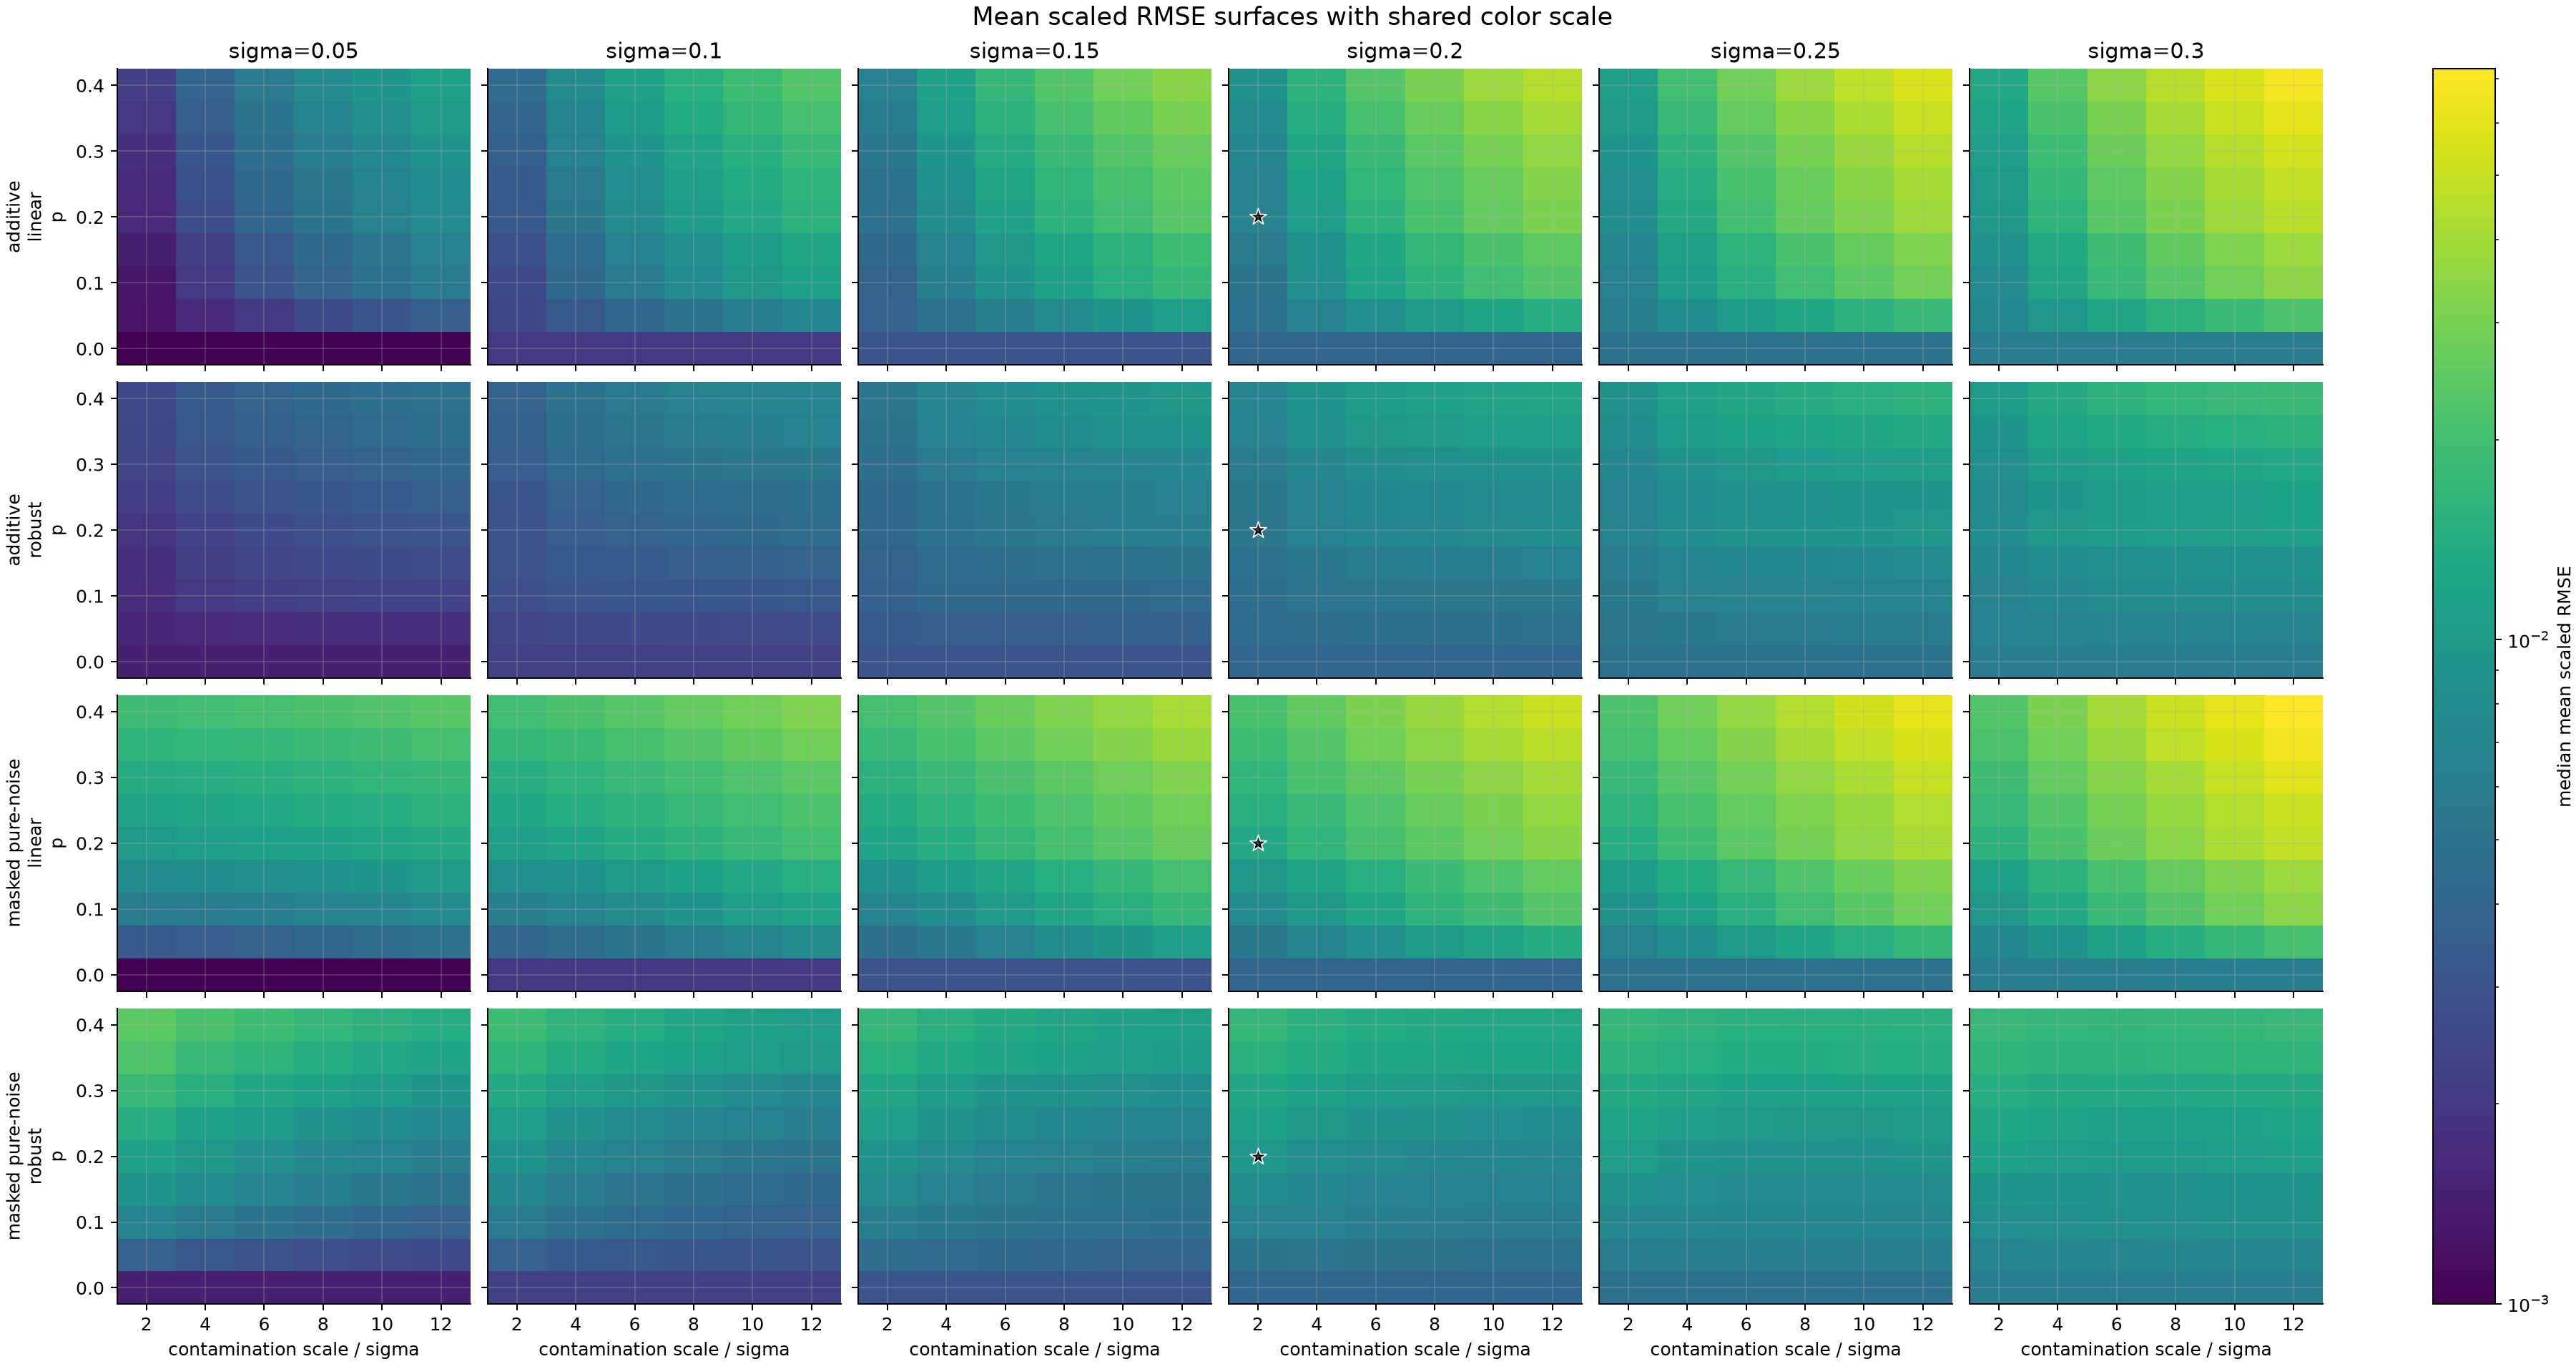
\includegraphics[width=\paperwidth,height=114mm,keepaspectratio]{irmf-talk/error_surfaces_cropped.png}}
    \par\vspace{-1mm}{\fontsize{9}{10}\selectfont\color{muted}Rows: additive / replaced (masked) contamination \(\times\) linear / IRMF. One colour scale; 324 settings \(\times\) 3 repeats.\par}
\end{frame}

\begin{frame}{Contamination probability and size at \(\sigma=0.2\)}
    \plot[68mm]{irmf-talk/slices_rmse_row.png}
    \vspace{1mm}
    Right: when contamination \emph{replaces} the signal (dashed red), IRMF's error \textcolor{teal}{decreases} as the contamination gets larger.
    \fignote{Median and IQR over 3 repeats. Confirmed with 100 repeats (backup): \(0.0093\) at \(2\sigma\) \(\to\) \(0.0082\) from \(6\sigma\) on.}
\end{frame}

\begin{frame}{Why larger contamination can help IRMF}
    \plot[72mm]{irmf-talk/toy_window.pdf}
    \vspace{1mm}
    A replaced point carries no signal. Linear IMF always averages it in: \(0.8\times\)truth.
    IRMF caps each point's pull. Small contamination looks like data and drags it toward 0; large contamination sits far
    on both sides, the capped pulls cancel, and IRMF effectively ignores those points.
    \fignote{One window: true value 0.4, \(\sigma=0.2\), \(H=0.4\), 20\% replaced by \(G+C\), \(C=\pm s\cdot\mathrm{Exp}(1)\); population estimates.}
\end{frame}

\begin{frame}{EMD: the standard data-driven decomposition}
    \vspace{-2mm}
    \plot[88mm]{irmf-talk/emd_sifting.pdf}
    \vspace{1mm}
    Empirical mode decomposition (Huang et al., 1998) repeats steps 1\textendash{}2 (\emph{sifting}) to peel off the finest component, then starts again on the rest.
    \fignote{No statistical model behind the steps; noise and spikes move the extrema, so scales can mix across components.}
\end{frame}

\begin{frame}{Real signals: two audio datasets}
    \begin{columns}[T,onlytextwidth]
        \begin{column}{0.48\textwidth}
            {\color{blue}\large BirdCLEF 2023}\par\vspace{2mm}
            16 bird species\par
            12,000 frames from 1,280 recordings\par
            451 recordists
        \end{column}
        \begin{column}{0.48\textwidth}
            {\color{orange}\large ESC-50 animals}\par\vspace{2mm}
            10 animal classes (dog, rooster, frog, \dots)\par
            5,100 frames from 400 clips\par
            157 uploaders
        \end{column}
    \end{columns}
    \vspace{6mm}
    Each frame: 2,048 samples (93 ms at 22 kHz).\par\vspace{3mm}
    Pipeline: frame \(\to\) EMD / linear IMF / IRMF \(\to\) simple statistics of each component
    (energy, spread, zero crossings, spectral centroid, \dots) \(\to\) linear classifier.
    \fignote{Cross-validation folds hold out whole recordists / uploaders, so the same recording never appears in training and test.}
\end{frame}

\begin{frame}{Real signals: IMF components beat EMD as features}
    \plot[62mm]{irmf-talk/classification_two_datasets.pdf}
    \vspace{1mm}
    IRMF beats EMD by \(+6.1\) pp (BirdCLEF) and \(+11.0\) pp (ESC-50) balanced accuracy.
    Against linear IMF there is no significant difference, so the gain over EMD comes from the IMF construction.
    \fignote{Fixed classifier: logistic regression (BirdCLEF), linear SVM (ESC-50); 5 grouped folds \(\times\) 3 seeds; Nadeau\textendash{}Bengio corrected 95\% CIs; filled = Holm \(p<0.05\).}
\end{frame}

\begin{frame}[fragile]{Software: \texttt{pimf}}
    NumPy-only Python library; linear and robust fits, parallel windows.
    \vspace{3mm}
\begin{semiverbatim}\small
pip install pimf

from pimf import IMF, SmoothAbs
res = IMF(SmoothAbs(H=0.4), solver="newton").decompose(y, k_max=9)
res.imfs, res.residual, res.stages
\end{semiverbatim}
\end{frame}

\begin{frame}{Why it works (1): the fit and its population target}
    For one component, with kernel weights \(w_{u,t}\defeq K_h(t-u)\):
    \[
        \widetilde S_t\defeq \arg\inf_z\sum_u\rho(Y_u-z)\,w_{u,t},\qquad
        S_t\defeq \arg\inf_z\sum_u\mathbb E\,\rho(Y_u-z)\,w_{u,t}.
    \]
    \(\widetilde S_t\) is the fit to the data; \(S_t\) is its \emph{population target}, the fit after averaging out the noise.
    With \(\phi(z)\defeq \mathbb E\,\rho(z+\varepsilon)\), curvature and centred score at the target are
    \[
        F_t\defeq \sum_u\phi''(X_u-S_t)\,w_{u,t},\quad D_t\defeq F_t^{1/2},\qquad
        \nabla_t\defeq \sum_u\bigl\{\rho'(Y_u-S_t)-\mathbb E\,\rho'(Y_u-S_t)\bigr\}w_{u,t}.
    \]
    \[
        \boxed{\widetilde S_t-S_t=\underbrace{F_t^{-1}\nabla_t}_{\text{leading random term}}+\underbrace{R_t}_{\text{remainder}}}
    \]
    \fignote{The identity defines \(R_t\). Independent errors with \(\mathbb E|\varepsilon_u|<\infty\); \(\rho\) convex, \(C^3\), with \(|\rho'|\le L_1\), \(0\le\rho''\le L_2\), \(|\rho'''|\le L_3\) (for \(\rho_H\): \(L_1=1\)).}
\end{frame}

\begin{frame}{Why it works (1) in pictures: fit vs.\ target}
    \plot[84mm]{irmf-talk/fit_vs_target.pdf}
    \vspace{1mm}
    Left: each noisy window has its own minimum \(\widetilde S_t\); they scatter around the minimum \(S_t\) of the averaged loss.
    Right: the error is almost exactly the leading term \(F_t^{-1}\nabla_t\); the remainder \(R_t\) is tiny.
    \fignote{One IRMF window of 15 points, \(\sigma=0.2\), \(H=0.4\); 14 draws on the left, 4,000 on the right (median \(|R_t|=0.0013\) vs.\ median error 0.046).}
\end{frame}

\begin{frame}{Why it works (2): Proposition 4.1}
    \textbf{Proposition 4.1.} Suppose that the conditions above hold and that
    \(\delta<1\) and \(\dfrac{C_1C_3}{D_{\min}(1-\delta)^2}<\dfrac49\).
    Then there is a random set \(\Omega(x)\) with \(\mathbb P\{\Omega(x)\}\ge1-e^{-x}\) such that
    \[
        \sup_{t\in\mathcal T_n}\bigl|D_t\bigl(\widetilde S_t-S_t-F_t^{-1}\nabla_t\bigr)\bigr|
        \le\frac{1}{D_{\min}}\Bigl\{\frac{9C_1^2C_3}{8(1-\delta)^3}+\frac{C_1C_2}{1-\delta}\Bigr\}.
    \]
    On the same event, every empirical minimizer is unique and
    \(\sup_{t\in\mathcal T_n}D_t|\widetilde S_t-S_t|\le\dfrac{3C_1}{2(1-\delta)}\).\par\vspace{4mm}
    {\color{muted}where, with \(z_x\defeq x+\log(4m)\), \(Q_t^2\defeq \sum_uw_{u,t}^2\), \(k_t\defeq \max_uw_{u,t}\), \(W_t\defeq \sum_uw_{u,t}\):}
    \[
        C_1\defeq \max_{t}\frac{L_1}{D_t}\Bigl\{Q_t\sqrt{2z_x}+\tfrac23k_tz_x\Bigr\},\quad
        C_2\defeq \max_{t}\frac{L_2}{D_t}\Bigl\{Q_t\sqrt{2z_x}+\tfrac13k_tz_x\Bigr\},\quad
        C_3\defeq \max_{t}\frac{L_3W_t}{D_t^2},\quad
        \delta\defeq \frac{C_2}{D_{\min}}.
    \]
    \fignote{Lemma 4.2: on \(\Omega(x)\), \(C_1\) bounds the centred score, \(C_2\) the curvature fluctuation and \(C_3\) the third derivative, simultaneously for all \(t\in\mathcal T_n\) (\(m\) evaluation points). Conditions: those on the previous slide.}
\end{frame}

\begin{frame}{Why it works (3): later components}
    \begin{itemize}
        \setlength{\itemsep}{4mm}
        \item \textbf{Linear IMF.} Component \(k\) sees the noise through
              \(e_k=W_{h_k}\prod_{j<k}(I-W_{h_j})\,\varepsilon\).
              For a positive-definite kernel each factor \(I-W_h\) is a contraction, so the error of
              component \(k\) stays at the noise level of its own window, \(\sigma/\sqrt{nh_k}\)
              \textemdash{} the \(a^{k/2}\) growth on slides 7\textendash{}8.
        \item \textbf{IRMF: even the second component is work in progress.} Its input residual
              \(Y-\widetilde S^{(1)}\) has noise that is no longer independent or Gaussian, so the
              first-component argument does not apply directly.
        \item \textbf{Draft idea.} Replace Bernstein by Gaussian concentration for Lipschitz functions;
              the hope is that the one-step rate \(\sqrt{z_x/(nh_2)}\) survives, up to a constant.
        \item \textbf{Open.} Components \(k\ge2\) for IRMF, and theory under contamination (current results assume Gaussian noise).
    \end{itemize}
    \fignote{With the periodic boundary all \(W_h\) commute, so \(\|e_k\|\le\|W_{h_k}\varepsilon\|\). The kernel matters: \(\|I-W_h\|\le1\) holds for \((1-|u|)_+^2\) (used here), not for Epanechnikov \(\tfrac34(1-u^2)_+\).}
\end{frame}

\begin{frame}{Summary}
    \begin{itemize}
        \setlength{\itemsep}{6mm}
        \item IMF splits a signal into scales by repeated local fits on residuals;
              IRMF keeps the recursion but caps how hard any single point can pull.
        \item Without contamination the two methods agree. With contamination IRMF follows the real components,
              and its error stays flat as the contamination grows: \textcolor{teal}{\(-75\%\)} vs.\ linear IMF at \(12\sigma\).
        \item When contamination replaces the signal, larger contamination even helps IRMF:
              clearly-off points are effectively ignored, subtle ones are not.
        \item On real audio (BirdCLEF, ESC-50), IMF components beat EMD features by 6\textendash{}11 pp.
        \item For the first component the fit concentrates around its population target (Proposition 4.1); later components are work in progress.
    \end{itemize}
    \fignote{\(-75\%\): mean scaled RMSE, 100 repeats, \(\sigma=0.2\), \(p=0.2\), both contamination models.}
\end{frame}

\appendix
\begin{frame}[plain]
    \vfill{\usebeamerfont{title}Backup\par}\vfill
\end{frame}

\begin{frame}{Backup: the sweep slice with 100 repeats}
    \plot[80mm]{irmf-talk/mc_slice_confirmation.pdf}
    \fignote{Same metric as slide 12 (mean over components of RMSE\(/a^{k/2}\)); median and IQR over 100 independent repeats.}
\end{frame}

\begin{frame}{Backup: component 1, replaced contamination}
    \plot[66mm]{irmf-talk/irmf_bias_variance_masked.pdf}
    \vspace{1mm}
    Error split over 100 repeats into a \emph{systematic shift} (the average error) and a \emph{random spread} around it.
    IRMF's shift shrinks toward the value obtained when the replaced points are removed; its spread levels off.
    Linear IMF keeps a fixed shift (20\% of the signal is missing) and its spread grows with contamination size.
\end{frame}

\begin{frame}{Backup: implementation details}
    \begin{itemize}
        \setlength{\itemsep}{3mm}
        \item Windows \(501,355,251,177,125,89,63,45,31\); periodic boundary; same weights for both methods.
        \item Implemented weights \(w(u)\propto(1-|u|)_+^2\) (the review calls them Epanechnikov).
        \item IRMF: \(H=2\sigma\), lookup-table score, gradient descent, at most 60 steps, tolerance \(10^{-6}\).
        \item Contamination \(C_i=\pm s\cdot\mathrm{Exp}(1)\) with a random sign; replaced (masked) model: \(Y_i=G_i+C_i\) at contaminated points.
        \item Slides 2\textendash{}3, 5\textendash{}8, 10: review signal and seed 777, \(\sigma=0.4\), \(p=0.2\), contamination scale \(6\sigma\).
        \item 100-repeat Monte Carlo: \(\sigma=0.2\), \(p=0.2\), \(H=0.4\), \(s/\sigma\in\{0.5,\dots,20\}\), notebook code unchanged.
    \end{itemize}
\end{frame}

\end{document}
